%review=doublespace preprint=single 5p=2 column
\documentclass[12pt,3p,authoryear]{elsarticle}

%% add packages %%
%% ------------ %%
\usepackage[hyphens]{url}
\usepackage{graphicx}
\usepackage{booktabs}
\usepackage[T1]{fontenc}
\usepackage{lmodern}
\usepackage{caption}
\usepackage{subfig}
\usepackage{amssymb, amsmath}
\usepackage[inline]{enumitem}
\usepackage{float}
\usepackage{tabularx}
\usepackage[dvipsnames, table]{xcolor}
\usepackage{ifxetex, ifluatex}
\usepackage{fixltx2e}
\usepackage[unicode=true, colorlinks]{hyperref}
\usepackage{cleveref}
\usepackage{tabu}
\usepackage{mathpazo}
%% ------------ %%

%% Conditional Packages %%
%% -------------------- %%



% use upquote if available, for straight quotes in verbatim environments
\IfFileExists{upquote.sty}{\usepackage{upquote}}{}

\ifnum 0\ifxetex 1\fi\ifluatex 1\fi=0 % if pdftex
  \usepackage[utf8]{inputenc}


\else % if luatex or xelatex
  \usepackage{fontspec}
  \ifxetex
    \usepackage{xltxtra,xunicode}
  \fi
  \defaultfontfeatures{Mapping=tex-text,Scale=MatchLowercase}
  \newcommand{\euro}{€}



    \setmonofont{sourcecodepro}


\fi

% use microtype if available
\IfFileExists{microtype.sty}{\usepackage{microtype}}{}




\usepackage{color}
\usepackage{fancyvrb}
\newcommand{\VerbBar}{|}
\newcommand{\VERB}{\Verb[commandchars=\\\{\}]}
\DefineVerbatimEnvironment{Highlighting}{Verbatim}{commandchars=\\\{\}}
% Add ',fontsize=\small' for more characters per line
\usepackage{framed}
\definecolor{shadecolor}{RGB}{248,248,248}
\newenvironment{Shaded}{\begin{snugshade}}{\end{snugshade}}
\newcommand{\KeywordTok}[1]{\textcolor[rgb]{0.13,0.29,0.53}{\textbf{#1}}}
\newcommand{\DataTypeTok}[1]{\textcolor[rgb]{0.13,0.29,0.53}{#1}}
\newcommand{\DecValTok}[1]{\textcolor[rgb]{0.00,0.00,0.81}{#1}}
\newcommand{\BaseNTok}[1]{\textcolor[rgb]{0.00,0.00,0.81}{#1}}
\newcommand{\FloatTok}[1]{\textcolor[rgb]{0.00,0.00,0.81}{#1}}
\newcommand{\ConstantTok}[1]{\textcolor[rgb]{0.00,0.00,0.00}{#1}}
\newcommand{\CharTok}[1]{\textcolor[rgb]{0.31,0.60,0.02}{#1}}
\newcommand{\SpecialCharTok}[1]{\textcolor[rgb]{0.00,0.00,0.00}{#1}}
\newcommand{\StringTok}[1]{\textcolor[rgb]{0.31,0.60,0.02}{#1}}
\newcommand{\VerbatimStringTok}[1]{\textcolor[rgb]{0.31,0.60,0.02}{#1}}
\newcommand{\SpecialStringTok}[1]{\textcolor[rgb]{0.31,0.60,0.02}{#1}}
\newcommand{\ImportTok}[1]{#1}
\newcommand{\CommentTok}[1]{\textcolor[rgb]{0.56,0.35,0.01}{\textit{#1}}}
\newcommand{\DocumentationTok}[1]{\textcolor[rgb]{0.56,0.35,0.01}{\textbf{\textit{#1}}}}
\newcommand{\AnnotationTok}[1]{\textcolor[rgb]{0.56,0.35,0.01}{\textbf{\textit{#1}}}}
\newcommand{\CommentVarTok}[1]{\textcolor[rgb]{0.56,0.35,0.01}{\textbf{\textit{#1}}}}
\newcommand{\OtherTok}[1]{\textcolor[rgb]{0.56,0.35,0.01}{#1}}
\newcommand{\FunctionTok}[1]{\textcolor[rgb]{0.00,0.00,0.00}{#1}}
\newcommand{\VariableTok}[1]{\textcolor[rgb]{0.00,0.00,0.00}{#1}}
\newcommand{\ControlFlowTok}[1]{\textcolor[rgb]{0.13,0.29,0.53}{\textbf{#1}}}
\newcommand{\OperatorTok}[1]{\textcolor[rgb]{0.81,0.36,0.00}{\textbf{#1}}}
\newcommand{\BuiltInTok}[1]{#1}
\newcommand{\ExtensionTok}[1]{#1}
\newcommand{\PreprocessorTok}[1]{\textcolor[rgb]{0.56,0.35,0.01}{\textit{#1}}}
\newcommand{\AttributeTok}[1]{\textcolor[rgb]{0.77,0.63,0.00}{#1}}
\newcommand{\RegionMarkerTok}[1]{#1}
\newcommand{\InformationTok}[1]{\textcolor[rgb]{0.56,0.35,0.01}{\textbf{\textit{#1}}}}
\newcommand{\WarningTok}[1]{\textcolor[rgb]{0.56,0.35,0.01}{\textbf{\textit{#1}}}}
\newcommand{\AlertTok}[1]{\textcolor[rgb]{0.94,0.16,0.16}{#1}}
\newcommand{\ErrorTok}[1]{\textcolor[rgb]{0.64,0.00,0.00}{\textbf{#1}}}
\newcommand{\NormalTok}[1]{#1}


\usepackage{longtable}




% Pandoc toggle for numbering sections (defaults to be off)
\setcounter{secnumdepth}{5}

%% Use Landscape Pages
\usepackage{lscape}

\usepackage{setspace}
\setstretch{1.5}

\usepackage{lmodern}

%% -------------------- %%

%% Create and Provide some customizations %%
%% -------------------------------------- %%
\providecommand{\tightlist}{%
  \setlength{\itemsep}{0pt}\setlength{\parskip}{0pt}}
  
%% Custom macros
\newtheorem{mydef}{Definition}
\newcommand{\bs}[1]{\ensuremath{\boldsymbol{#1}}}
\newcommand{\diag}[1]{\mathrm{diag}\left(#1\right)}
\newcommand{\seq}[3][1]{\ensuremath{#2_{#1},\ldots,\,#2_{#3}}}
\newcommand{\note}[1]{\marginpar{\scriptsize\tt{\color{RoyalBlue}#1}}}
\newcommand{\edit}[1]{{\color{OrangeRed} #1}}

% set some lengths
\setlength{\parindent}{0pt}
% \setlength{\parskip}{6pt plus 2pt minus 1pt}
\setlength{\emergencystretch}{3em}  % prevent overfull lines

%% Hyperref color setup
\AtBeginDocument{%
  %% Define Colors
  \newcommand\myshade{80}
  \colorlet{mylinkcolor}{violet!\myshade!black}
  \colorlet{mycitecolor}{YellowOrange!\myshade!black}
  \colorlet{myurlcolor}{Aquamarine!\myshade!black}

  \hypersetup{
    breaklinks = true,
    bookmarks  = true,
    pdfauthor  = {},
    pdftitle   = {Comparison of Multivariate Estimation Methods},
    linkcolor  = mylinkcolor,
    citecolor  = mycitecolor,
    urlcolor   = myurlcolor,
    colorlinks = true,
  }
}
\urlstyle{same}  % don't use monospace font for urls
%% -------------------------------------- %%

%% Customizations %%
%% -------------- %%
 % turn line numbering on

%% -------------- %%

%% Configure Bibliography %%
%% ---------------------- %%
\bibliographystyle{elsarticle-harv}
\biboptions{square}

% \makeatletter
% \providecommand{\doi}[1]{%
%   \begingroup
%     \let\bibinfo\@secondoftwo
%     \urlstyle{rm}%
%     \href{http://dx.doi.org/#1}{%
%       doi:\discretionary{}{}{}%
%       \nolinkurl{#1}%
%     }%
%   \endgroup
% }
% \makeatother

% 

%% Header Includes %%
%% --------------- %%
%% --------------- %%



\begin{document}
%% --- Front Matter Start --- %%
\begin{frontmatter}

  \title{Comparison of Multivariate Estimation Methods}
  
    \author[KBM]{Raju Rimal\corref{c1}}
   \ead{raju.rimal@nmbu.no} 
   \cortext[c1]{Corresponding Author}
    \author[KBM]{Trygve Almøy}
   \ead{trygve.almoy@nmbu.no} 
  
    \author[NMBU]{Solve Sæbø}
   \ead{solve.sabo@nmbu.no} 
  
      \address[KBM]{Faculty of Chemistry and Bioinformatics, Norwegian University of Life
Sciences, Ås, Norway}
    \address[NMBU]{Prorector, Norwegian University of Life Sciences, Ås, Norway}
  
  \begin{abstract}
  While Data science is battling to extract information from enormous
  explosion of data, many estimators and algorithms are being developed
  for better prediction. Researchers and data scientists often introduce
  new methods and evaluate them based on various aspects of data. However,
  these studies seldom study the impact of/on multiple response model.
  This study compares some newly-developed (envelope estimation) and
  well-established estimators (PLS, PCR, Ridge and Lasso) based on the
  simulated data specifically designed by variying properties such as
  multicollinearity, correlation between multiple response and amount of
  information content in latent variables. This study aims to identify
  itself as an additional eye for researcher to look at these methods.
  \end{abstract}
   \begin{keyword} model-comparison,multi-response,simrel\end{keyword}

\end{frontmatter}

\section{Introduction}\label{introduction}

``Big Data'' is becoming a focal discussion in many discipline. Massive
explosion of data, integrated with information in several variables and
features, have made exploration and analysis more difficult. Researchers
are devising new methods and algorithms in order to extract such
information weather to study the relationship between variables or to
create a predictive model. Mostly, the models used for study contains
predictor variables that are directly or indirectly correlated with
other predictor variables and many response variables. These interlinked
relationship observed as a nature of data influences any study whether
it is a predictive modeling or an inference.

Modern inter-disciplinary research fields such as chemometrics,
echonometrics and bioinformatics are handling multi-response models
extensively. This paper attempts to compare some of such methods and
their performance on linear model data with specifically designed
properties. The properties includes coefficient of determination,
correlation between response variables, correlation between predictor
variables and number of predictor variables. These properties are
discussed more in \protect\hyperlink{experimental-design}{Experimental
Design} section.

\citet{saebo2015simrel} and \citet{Alm_y_1996} have made similar
comparison with single response setting. \citet{Rimal_2018} has
introduced a method for simulating multi-response data based on data
properties as parameters. The study also has made a basic comparison on
some estimation methods and their interaction with the data properties
of a multi-response model. The main aim of this paper is to present a
comprehensive comparison of contemporary estimation methods with
customary estimation methods using dataset simulated with particular
properties. An experimental design and the methods under comparison are
discussed followed by a brief discussion of strategy behind the data
simulation.

\section{Simulation Model}\label{simulation-model}

Consider a model where response variable \((\mathbf{y})\) and predictor
variable \((\mathbf{x})\) follows normal distribution as follows,

\begin{equation}
  \begin{bmatrix}
    \mathbf{y} \\ \mathbf{x}
  \end{bmatrix} \sim \mathbf{N}
  \left(
    \begin{bmatrix}
      \boldsymbol{\mu}_y \\
      \boldsymbol{\mu}_x
    \end{bmatrix},
    \begin{bmatrix}
    \boldsymbol{\Sigma}_{yy} & \boldsymbol{\Sigma}_{yx} \\
    \boldsymbol{\Sigma}_{xy} & \boldsymbol{\Sigma}_{xx}
    \end{bmatrix}
  \right)
  \label{eq:model-1}
\end{equation}

where, \(\boldsymbol{\Sigma}_{yy}\) is the variance-covariance matrix of
\(\mathbf{y}\) and \(\boldsymbol{\Sigma}_{xx}\) is the
variance-covariance matrix of \(\mathbf{x}\). The covariance between
\(\mathbf{x}\) and \(\mathbf{y}\) is \(\boldsymbol{\Sigma}_{xy}\).
\(\boldsymbol{\mu}_y\) and \(\boldsymbol{\mu}_x\) are mean vector of
\(\mathbf{x}\) and \(\mathbf{y}\) respectively. An equivalent regression
model of \eqref{eq:model-1} can be defined as,

\begin{equation}
\mathbf{y} = \mu_y + \boldsymbol{\beta}^t(\mathbf{x} - \mu_x) + \epsilon
\label{eq:reg-model-1}
\end{equation}

where, \(\boldsymbol{\beta}^t\) is a matrix of regression coefficients
and \(\epsilon\) is an error term such that
\(\epsilon \sim N(0, \Sigma_{y|x})\)

In a casual relationship model like \eqref{eq:reg-model-1}, we assume that
the variation in response \(\mathbf{y}\) is caused by the predictor
\(\mathbf{x}\). However, in many situations, only small proportion of
the variation in \(\mathbf{x}\) have some connection with
\(\mathbf{y}\). This space can be referred as relevant or material space
of \(\mathbf{x}\) and rest as irrelevant or immaterial space. In the
similar manner, we can assume that only some part of variation in
\(\mathbf{y}\) is caused by the predictors or contains the information
(Figure-\ref{fig:relevant-space}). Following the concept of relevant and
irrelevant space \textbf{(Helland \& Trygve, 1994)}, a set of latent
variables (such as principal components) that spans these space can be
imagined in both predictors and response space. Let us consider the
components that spans the relevant predictor space as predictor
components and the components that spans the relevant response space as
response components. Further let us define the components that spans the
irrelevant space as irrelevant components.

\begin{figure}

{\centering 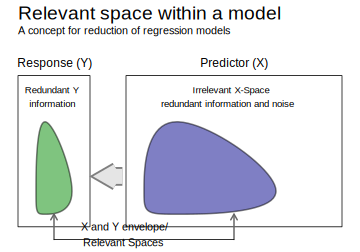
\includegraphics[width=0.8\linewidth]{main_files/figure-latex/relevant-space-1} 

}

\caption{Relevant space in a regression model}\label{fig:relevant-space}
\end{figure}

Estimation methods like Partial Least Square Regression and many of its
derivetives have been using the idea of relevant components in predictor
space for better estimation and prediction (\emph{perhaps need
citation}). More recent methods such as Simultaneous Envelope
\citep{cook2015simultaneous} have extended the concept to formulate
informative response space (envelope) to decrease error variance in both
prediction and estimation.

\begin{center}\rule{0.5\linewidth}{\linethickness}\end{center}

Define a transformation \(\mathbf{w} = \mathbf{Qy}\) and
\(\mathbf{z} = \mathbf{Rx}\) such that \(\mathbf{Q}\) and \(\mathbf{R}\)
are orthogonal rotation matrix which transform \(\mathbf{x}\) and
\(\mathbf{y}\) into latent components \(\mathbf{z}\) and \(\mathbf{w}\)
respectively. An equivalent model to \eqref{eq:model-1} can be defined as,

\begin{equation}
  \begin{bmatrix}
    \mathbf{w} \\ \mathbf{z}
  \end{bmatrix} \sim \mathbf{N}
  \left(
    \begin{bmatrix}
      \boldsymbol{\mu}_w \\
      \boldsymbol{\mu}_z
    \end{bmatrix},
    \begin{bmatrix}
    \boldsymbol{\Sigma}_{ww} & \boldsymbol{\Sigma}_{wz} \\
    \boldsymbol{\Sigma}_{zw} & \boldsymbol{\Sigma}_{zz}
    \end{bmatrix}
  \right) = \mathbf{N}
  \left(
    \begin{bmatrix}
      \mathbf{Q}\boldsymbol{\mu}_w \\
      \mathbf{R}\boldsymbol{\mu}_z
    \end{bmatrix},
    \begin{bmatrix}
    \mathbf{Q}\boldsymbol{\Sigma}_{ww}\mathbf{Q}^t & \mathbf{Q}\boldsymbol{\Sigma}_{wz}\mathbf{R}^t \\
    \mathbf{R}\boldsymbol{\Sigma}_{zw}\mathbf{Q}^t & \mathbf{R}\boldsymbol{\Sigma}_{zz}\mathbf{R}^t
    \end{bmatrix}
  \right)
  \label{eq:model-2}
\end{equation}

Here, \(\mathbf{w}\) and \(\mathbf{z}\) can be considered as principal
components of response (response components) and predictors (predictor
components) respectively. A regression model equivalent to
\eqref{eq:model-2} can be defined as,

\begin{equation}
\mathbf{w} = \mu_w + \boldsymbol{\alpha}^t(\mathbf{z} - \mu_z) + \tau
\label{eq:reg-model-2}
\end{equation}

where, \(\boldsymbol{\alpha}^t\) is a matrix of regression coefficients
and \(\tau\) is an error term such that \(\tau \sim N(0, \Sigma_{w|z})\)

\emph{\textbf{If we should write this part perhaps we should describe
how data are simulated from the model above}}

\begin{center}\rule{0.5\linewidth}{\linethickness}\end{center}

In this study, data is simulated based on model-\eqref{eq:model-1} using
an R-package ``\texttt{simrel}''. \citet{Rimal_2018} has discussed the
concept behind the simulation in detail that is implemented in the
R-package. Properties in the simulated data such as its dimension,
correlation structure and signal-to-noise ratio are controlled through
parameters. The estimation methods under comparison, discussed in
\protect\hyperlink{methods}{Methods} section, are tested against these
dataset and evaluated on the basis of their performance on both
prediction and estimation.

\hypertarget{experimental-design}{\section{Experimental
Design}\label{experimental-design}}

A complete factorial design with different levels of parameters are used
as follows.

\begin{description}
\tightlist
\item[\textbf{Number of predictors:}]
In order to observe the performance of estimators on tall and wide
predictor matrices, 20 and 250 predictor variables are simulated.
Parameter \texttt{p} controls this properties in \texttt{simrel}
function in the R Package.
\item[\textbf{Multicollinearity in predictor variables:}]
Highly collinear predictors can be explained completely by few
components. Parameter \texttt{gamma} (\(\gamma\)) in \texttt{simrel}
controls the eigenvalues of the predictor variables as \eqref{eq:gamma}.

\begin{equation}
  \lambda_i = e^{-\gamma(i - 1), \gamma > 0} \text{ and } i = 1, 2, \ldots, p
  \label{eq:gamma}
  \end{equation}

Here, \(\lambda_i, i = 1, 2, \ldots p\) are eigenvalues of predictor
variables. Here we have used 0.2 and 0.9 as different levels of
\texttt{gamma}. Higher the value of gamma, higher will be the
correlation between predictors and vice versa.
\item[\textbf{Correlation in response variables:}]
Correlation in response variables is less explored area. Here we have
tried to explore that part with 4 levels of correlation in response
variables. We have used \texttt{eta} \(\eta\) parameter of
\texttt{simrel} for controlling the eigenvalues corresponding to
response variables as \eqref{eq:eta}.

\begin{equation}
  \kappa_i = e^{-\eta(i - 1), \eta > 0} \text{ and } j = 1, 2, \ldots, m
  \label{eq:eta}
\end{equation}

Here, \(\kappa_i, i = 1, 2, \ldots m\) are eigenvalues of response
variables and \texttt{m} is number of response variables. Here we have
used 0, 0.4, 0.8 and 1.2 as different levels of \texttt{eta}. Larger the
value of eta, larger will be the correlation between response variables
and vice versa.
\item[\textbf{Coefficient of determination:}]
Coefficient of determination controls signal-to-noise ratio in simulated
data and influence the prediction heavily. \texttt{R2} parameters in
\texttt{simrel} package is used to specify coefficient of determination
correlation for a response components. Here we have used single response
component which contains information for the relevant predictor
components. The single informative response components is \emph{blended}
in \texttt{m} response variables. Here we have used 0.8 and 0.8 levels
of coefficient of determination \texttt{R2} (\(\rho^2\)) corresponding
to the single response component.
\end{description}

Further, a complete factorial design from the levels of above parameters
gave us 32 designs. Each design is associated with a dataset having
unique properties. Table\textasciitilde{}\ref{tab:design-table}, shows
all the design obtained from above factors. For each design and
estimation method, 50 datasets were simulated for replication. In total,
there were \(7 \times 32 \times 50\), i.e.~11200 dataset simulated.

\begin{table}

\caption{\label{tab:design-table}Simulation parameters of all designs}
\centering
\begin{tabu} to \linewidth {>{\bfseries}r>{\raggedleft}X>{\raggedleft}X>{\raggedleft}X>{\raggedleft}X>{\bfseries}r>{\raggedleft}X>{\raggedleft}X>{\raggedleft}X>{\raggedleft}X}
\toprule
Design & p & eta & gamma & R2 & Design & p & eta & gamma & R2\\
\midrule
1 & 20 & 0.0 & 0.2 & 0.8 & 17 & 20 & 0.4 & 0.2 & 0.8\\
2 & 20 & 0.8 & 0.9 & 0.8 & 18 & 20 & 1.2 & 0.9 & 0.8\\
3 & 250 & 0.8 & 0.9 & 0.8 & 19 & 250 & 1.2 & 0.9 & 0.8\\
4 & 250 & 0.0 & 0.2 & 0.8 & 20 & 250 & 0.4 & 0.2 & 0.8\\
5 & 20 & 0.8 & 0.2 & 0.8 & 21 & 20 & 1.2 & 0.2 & 0.8\\
\addlinespace
6 & 20 & 0.0 & 0.9 & 0.8 & 22 & 20 & 0.4 & 0.9 & 0.8\\
7 & 250 & 0.0 & 0.9 & 0.8 & 23 & 250 & 0.4 & 0.9 & 0.8\\
8 & 250 & 0.8 & 0.2 & 0.8 & 24 & 250 & 1.2 & 0.2 & 0.8\\
9 & 20 & 0.0 & 0.9 & 0.8 & 25 & 20 & 0.4 & 0.9 & 0.8\\
10 & 20 & 0.8 & 0.2 & 0.8 & 26 & 20 & 1.2 & 0.2 & 0.8\\
\addlinespace
11 & 250 & 0.8 & 0.2 & 0.8 & 27 & 250 & 1.2 & 0.2 & 0.8\\
12 & 250 & 0.0 & 0.9 & 0.8 & 28 & 250 & 0.4 & 0.9 & 0.8\\
13 & 20 & 0.8 & 0.9 & 0.8 & 29 & 20 & 1.2 & 0.9 & 0.8\\
14 & 20 & 0.0 & 0.2 & 0.8 & 30 & 20 & 0.4 & 0.2 & 0.8\\
15 & 250 & 0.0 & 0.2 & 0.8 & 31 & 250 & 0.4 & 0.2 & 0.8\\
16 & 250 & 0.8 & 0.9 & 0.8 & 32 & 250 & 1.2 & 0.9 & 0.8\\
\bottomrule
\end{tabu}
\end{table}

\begin{description}
\tightlist
\item[\textbf{Common parameters:}]
Each dataset was simulated with \(n = 100\) number of observation and
\(m = 4\) response variables. Further, the position of relevant
predictor components are set to at position 1, 2, 3, 4 and 5, 6, 7, 8.
In addition, we have assumed that there is only 1 number of informative
response component. So, that the first informative response component is
rotated orthogonally together with 3 uninformative response components.
This spread out the information in all simulated response variables. For
further details see: \citep{Rimal_2018}.
\end{description}

An example of simulation parameters for the first design is as follows:

\begin{Shaded}
\begin{Highlighting}[]
\KeywordTok{simrel}\NormalTok{(}
  \DataTypeTok{n      =}\NormalTok{ 100L,                  ## Observations}
  \DataTypeTok{p      =}\NormalTok{ 20L,                   ## Predictors}
  \DataTypeTok{m      =}\NormalTok{ 4L,                    ## Response}
  \DataTypeTok{q      =} \DecValTok{20}\NormalTok{,                    ## Relevant predictors}
  \DataTypeTok{relpos =} \KeywordTok{list}\NormalTok{(}\KeywordTok{c}\NormalTok{(}\DecValTok{1}\NormalTok{, }\DecValTok{2}\NormalTok{, }\DecValTok{3}\NormalTok{, }\DecValTok{4}\NormalTok{)),   ## Position of predictor components}
  \DataTypeTok{eta    =} \DecValTok{0}\NormalTok{,                     ## Decay factor of response eigenvalues}
  \DataTypeTok{gamma  =} \FloatTok{0.2}\NormalTok{,                   ## Decay factor of predictor eigenvalues}
  \DataTypeTok{R2     =} \FloatTok{0.8}\NormalTok{,                   ## Coefficient of determination}
  \DataTypeTok{ypos   =} \KeywordTok{list}\NormalTok{(}\KeywordTok{c}\NormalTok{(}\DecValTok{1}\NormalTok{, }\DecValTok{2}\NormalTok{, }\DecValTok{3}\NormalTok{, }\DecValTok{4}\NormalTok{)), }
  \DataTypeTok{type   =} \StringTok{"multivariate"}
\NormalTok{)}
\end{Highlighting}
\end{Shaded}

Figure \ref{fig:est-cov-plot} shows the covariance structure of this
design. The left plot shows that only first four predictor components at
position 1, 2, 3 and 4 have high covariance with first response
components. Remaining predictor components are not relevant for any of
the response components and since response space is explained by single
components, response components except 1 has zero covariance with the
predictors components. This is the population covariance structure of
the simulated. The right plot, where as, shows that the all the
predictor components have non-zero covariance with all the response
components where first few components have large covariance than the
later components. The \texttt{eta} parameters controls the eigenvalues
corresponding to response variables, it should be relatively easier to
predict fourth response than first since it has less variation present
in the data and will be easier to explain by the predictors. This is
explored in \protect\hyperlink{analysis}{analysis} section of this
paper.

\begin{figure}
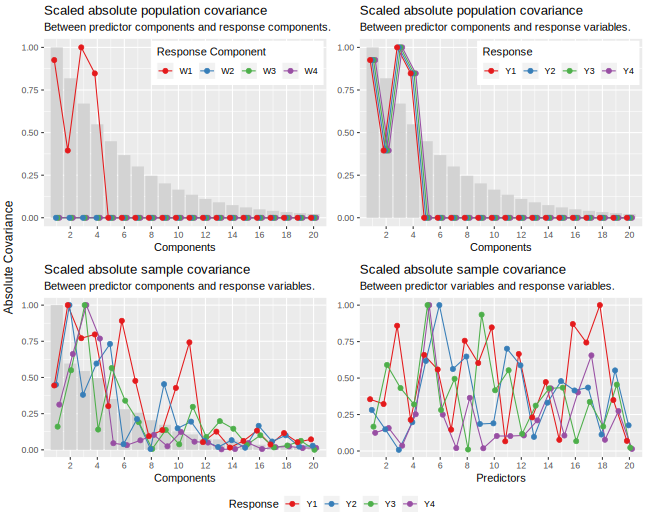
\includegraphics[width=1\linewidth]{main_files/figure-latex/est-cov-plot-1} \caption{Scaled covariance between predictor components and response components (left) and scaled expected covariance between predictor components and response variables (the one we obtain after rotation). The bar in the background eigenvalues corresponding to each components.}\label{fig:est-cov-plot}
\end{figure}

\hypertarget{methods}{\section{Methods}\label{methods}}

The aim of this paper is to compare some customary methods such as
Principal Component Regression (PCR), Partial Least Squares (PLS), Ridge
and Lasso with some stat-of-the-art methods such as envelope estimation
and simultaneous envelope estimation. This will also make comparison on
the methods based on reduced regression such as PCR, PLS and envelope
with that of Shrinkage methods such as Ridge and Lasso. The estimation
methods used for comparison as follows.

\begin{enumerate}
\def\labelenumi{\alph{enumi})}
\tightlist
\item
  Principal Component Regression (PCR)
\item
  Partial Least Squares Regression using single response per model
  (PLS1)
\item
  Partial Least Squares Regression using all response together (PLS2)
\item
  Ridge Regression
\item
  Lasso Regression
\item
  Envelope estimation in predictor space
  (Xenv)\citep{cook2015foundations}
\item
  Simultaneous estimation of envelope in both predictor and response
  space (Senv)\citep{cook2015simultaneous}
\end{enumerate}

\subsection{Modification in envelope
estimation}\label{modification-in-envelope-estimation}

Since envelope estimators (Xenv and Senv) are based on maximum
likelihood estimation (MLE), it fails to estimate on wide matrices, i.e.
\(p > n\). In order to incorporate these method in our comparison, we
have used the principal components \((\mathbf{z})\) of predictor
variables \((\mathbf{x})\) using required number of components for
capturing 97.5\% of the variation in it. The new set of variables
\(\mathbf{z}\) were used for envelope estimation. The regression
coefficients \((\hat{\boldsymbol{\alpha}})\) corresponding to these new
variables \(\mathbf{z}\) were transformed back to obtain coefficients
for each predictor variables \((\boldsymbol{\hat{\beta}})\) as,

\[\hat{\boldsymbol{\beta}} = \mathbf{e}_k\hat{\boldsymbol{\alpha}_k}\]
where, \(\mathbf{e}_k\) is the eigenvectors with \(k\) number of
components.

\subsection{Comparison Criteria}\label{comparison-criteria}

The models are compared on following three basis.

\begin{description}
\tightlist
\item[Estimation Error]
Diagonal elements of \eqref{eq:est-error} is used as estimation error of
each response in every fitted model.

\begin{equation}
  \text{estimation error} = \left(\boldsymbol{\beta} - \boldsymbol{\hat{\beta}}\right)^t\left(\boldsymbol{\beta} - \boldsymbol{\hat{\beta}}\right)
  \label{eq:est-error}
  \end{equation}

where, \(\boldsymbol{\beta}\) and \(\boldsymbol{\hat{\beta}}\) are true
and estimated regression coefficient corresponding to \eqref{eq:model-1}.
\item[Prediction Error]
Diagonal elements of \eqref{eq:pred-error} is used as estimation error of
each response in every fitted model.
\end{description}

\begin{equation}
\text{prediction error} = \left(\boldsymbol{\beta} - \boldsymbol{\hat{\beta}}\right)^t\Sigma_{xx}\left(\boldsymbol{\beta} - \boldsymbol{\hat{\beta}}\right) + \Sigma_{y|x}
\label{eq:pred-error}
\end{equation}

where, \(\Sigma_{xx}\) is the true covariance matrix of predictor and
\(\Sigma_{y\mid x}\) is the true model error both obtained from
simulation.

\begin{description}
\tightlist
\item[Comparison of estimated coefficients with true coefficients]
A graphical comparison of estimated coefficient from different
estimators is compared with the true coefficients. (\emph{need some
statistical way of doing so}) This shows how each additional components
contributes on finding beta coefficients closer to the true value. This
also helps us to see if the additional components contains noise how the
estimates deviates from the true coefficients.
\end{description}

\hypertarget{analysis}{\section{Analysis}\label{analysis}}

In order to carry out a proper statistical comparison, a multivariate
linear model is used with prediction and estimation error with respect
to each response variables as dependent variables and the interaction of
simulation parameters (\texttt{p}, \texttt{gamma}, \texttt{eta} and
\texttt{R2}) and \texttt{Methods} as independent variables as
\eqref{eq:full-model}.

\begin{equation}
\mathbf{y} = \boldsymbol{\mu} + \texttt{p} \times \texttt{gamma} \times \texttt{eta} \times \texttt{R2} \times \texttt{Methods} + \boldsymbol{\varepsilon}
\label{eq:full-model}
\end{equation}

where, \(y_j\) is the prediction error in one model and estimation error
in another corresponding to response \(j\). Let us discuss the results
of Multivariate Analysis of Variance (MANOVA) for both of these models.

\subsection{Prediction error model:}\label{prediction-error-model}

Using the prediction error corresponding to response \(j\) as \(y_j\) in
\eqref{eq:full-model} a 2nd interaction of methods and simulation
parameters as predictors, a clear high F-statistic corresponding to
Pillai statistic for coefficient of determination (\texttt{R2}) has
suggested high influence of \texttt{R2} in the model. In order to look
for effects of other interactions, we have used model
\eqref{eq:separate-pred-model} fitted for low and high coefficient of
determination separately.

\begin{equation}
\mathbf{y} = \boldsymbol{\mu} + \texttt{p} \times \texttt{gamma} \times \texttt{eta} \times \texttt{Methods} + \boldsymbol{\varepsilon}
\label{eq:separate-pred-model}
\end{equation}

From the ANOVA tables \ref{tab:pred-aov-R2-high} and
\ref{tab:pred-aov-R2-low}, we can see that the factor \texttt{eta} has
high effect on prediction error in both the cases of low and high
coefficient of determination. Also, Also, the tables show that Methods
have significantly large second and third order interaction with
\texttt{gamma} and \texttt{eta}, however this is mostly dominated by the
high main effect of \texttt{eta} which is same in both the models.









Although, methods have similar prediction performance for different
levels of \texttt{eta}, \texttt{R2} and \texttt{p}, the difference is
considerable for low and high multicollinearity in case of both low
(Figure \ref{fig:gamma-eff-pred-R2-low}) and high (Figure
\ref{fig:gamma-eff-pred-R2-high}) \texttt{R2}.

\subsection{Estimation error}\label{estimation-error}

\textbf{Some plots and descriptions on estimation error models}

Based on the simulation design and ANOVA analysis, following analysis
revolves abound the inter-connection between both prediction and
estimation errors and the properties of data. The analysis is based on
comparison of true and estimated regression coefficients, estimation
error and the prediction error. Following four groups can be identified
from the simulation design (see table \ref{tab:design-table}):

\begin{enumerate}
\def\labelenumi{\alph{enumi})}
\tightlist
\item
  Wide vs Tall prediction matrix (20 and 250)
\item
  High vs low multicollinearity (0.2 and 0.9)
\item
  High vs low coefficient of determination (0.8 and 0.8)
\item
  Different levels of correlation between responses (0, 0.4, 0.8 and
  1.2)
\end{enumerate}

\subsection{Error (prediction and estimation)
Analysis}\label{error-prediction-and-estimation-analysis}

\subsection{Regression Coefficients}\label{regression-coefficients}

\section{Discussion}\label{discussion}

\section*{References}\label{references}
\addcontentsline{toc}{section}{References}

\hypertarget{refs}{}

\appendix



\renewcommand\refname{References}
\bibliography{ref-db.bib}


\end{document}
